\begin{figure}[htbp]
\centering
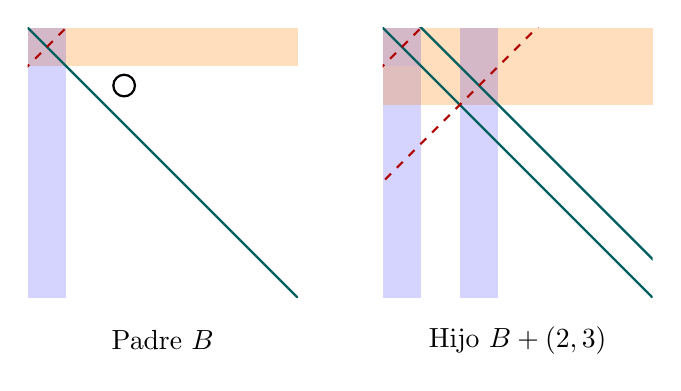
\begin{tikzpicture}[x=.49cm,y=.49cm]
 \foreach \etapa/\dx in {1/0,2/9.2}{
  \begin{scope}[shift={(\dx,0)}]
   \bcuadricula{7}
   \fill[orange,opacity=.26] (0,6) rectangle (7,7);
   \fill[blue,opacity=.17] (0,0) rectangle (1,7);
   \ifnum\etapa=2
    \fill[orange,opacity=.26] (0,5) rectangle (7,6);
    \fill[blue,opacity=.17] (2,0) rectangle (3,7);
   \fi
   \begin{scope}
    \clip (0,0) rectangle (7,7);
    \draw[teal!75!black,line width=.8pt] (.5,6.5) ++(-7,7) -- ++(14,-14);
    \draw[red!70!black,dashed,line width=.8pt] (.5,6.5) ++(-7,-7) -- ++(14,14);
    \ifnum\etapa=2
     \draw[teal!75!black,line width=.8pt] (2.5,5.5) ++(-7,7) -- ++(14,-14);
     \draw[red!70!black,dashed,line width=.8pt] (2.5,5.5) ++(-7,-7) -- ++(14,14);
    \fi
   \end{scope}
   \foreach \rr in {1,...,7}{
    \foreach \cc in {1,...,7}{
     \pgfmathtruncatemacro{\libre}{(\rr!=1)&&(\cc!=1)&&(abs(\rr-1)!=abs(\cc-1))}
     \ifnum\etapa=2
      \pgfmathtruncatemacro{\libre}{\libre&&(\rr!=2)&&(\cc!=3)&&(abs(\rr-2)!=abs(\cc-3))}
     \fi
     \ifnum\libre=1 \bmarca{7}{\rr}{\cc}\fi
    }
   }
   \breina{7}{1}{1}
   \ifnum\etapa=1
    \draw[black,line width=.8pt] (2.5,5.5) circle[radius=.28];
    \node at (3.5,-1.1) {Padre $B$};
   \else
    \breina{7}{2}{3}
    \node at (3.5,-1.1) {Hijo $B+(2,3)$};
   \fi
  \end{scope}
 }
\end{tikzpicture}
\caption{Una transición de un padre a un hijo en un tablero de orden siete. El padre tiene una reina
en la fila 1 y el hijo se obtiene al revelar la fila 2.
Las filas se numeran desde uno de arriba abajo y las columnas desde uno de izquierda a derecha.
Las coronas representan las reinas colocadas. Las bandas horizontales y verticales señalan sus filas y
columnas ocupadas. Las líneas continuas y discontinuas trazan las dos familias diagonales atacadas.
Cada punto indica una casilla disponible. En la fila siguiente, la $2$, las columnas $3,4,5,6,7$
tienen respectivamente $1,1,1,1,0$ completaciones, de modo que $Q(B)=4$. El círculo señala la elección
$(2,3)$ que produce el hijo de la derecha.}\label{fig:historia}
\end{figure}
